\chapter{Wstęp}

Radiologia zajmuje się obrazowaniem ciała człowieka z wykorzystaniem zjawisk fizycznych umożliwiających nieinwazyjny wgląd wewnątrz organizmu. Z uwagi \linebreak na szerokie możliwości diagnozowania chorób z wykorzystaniem radiologii, dziedzina ta ma coraz większe znaczenie w medycynie. Z danych przedstawionych przez Siemens Healthineers w 2018 roku wynika, że w ciągu ostatniej dekady liczba skanów z wykorzystaniem Tomografii Komputerowej i Rezonansu Magnetycznego zwiększa się co roku o 10--12\%. Jak wynika z katalogu ambulatoryjnych świadczeń diagnostycznych Narodowego Funduszu Zdrowia w Polsce, w roku 2018 było to około 1 mln skanów Rezonansu Magnetycznego i około 4 mln. Tomografii Komputerowych. Do tego należy doliczyć inne modalności jak klasyczne badanie rentgenowskie, czy Pozytonową Tomografię Emisyjną. Firmy badawcze np. PMR Consulting\&Researh wskazują, że w Europie, w tym w szczególności w Polsce, dokonuje się dużych inwestycji infrastrukturalnych, które dalej implikować będą wzrost liczby obrazowań.
  
Z danych przedstawionych przez Siemens Healthineers wynika również, że wzrost liczby radiologów nie przekracza 3\% rocznie. W zestawieniu z dynamiką liczby obrazowań, rezultatem jest zmniejszenie o połowę dostępnego czasu na opis pacjenta i wzrost błędu interpretacji badań nawet o 16,6 punktu procentowego, z czego 74\% wynika ze skutków przemęczenia i zaburzeń percepcji radiologów.  

Powyższy problem indukuje potrzebę rozwoju narzędzi wspomagających radiologów, a w szczególności pozwalających na automatyzację żmudnych, powtarzalnych zadań. Przewidywania wielu firm m.in. prestiżowej agencji PricewaterhouseCoopers (PwC) wskazują, że radiologia zostanie zrewolucjonizowana w najbliższych latach przez rozwiązania do komputerowego wspomagania, z emfazą na aplikacje wykorzystujące metody sztucznej inteligencji. Przewidywania te wyrażone\linebreak w udziale w produkcie krajowym brutto zastosowań metod Sztucznej Inteligencji (SI) można zaobserwować na Rys. \ref{MedTechGrowth}. 
\begin{figure}[h!]
	\centering
	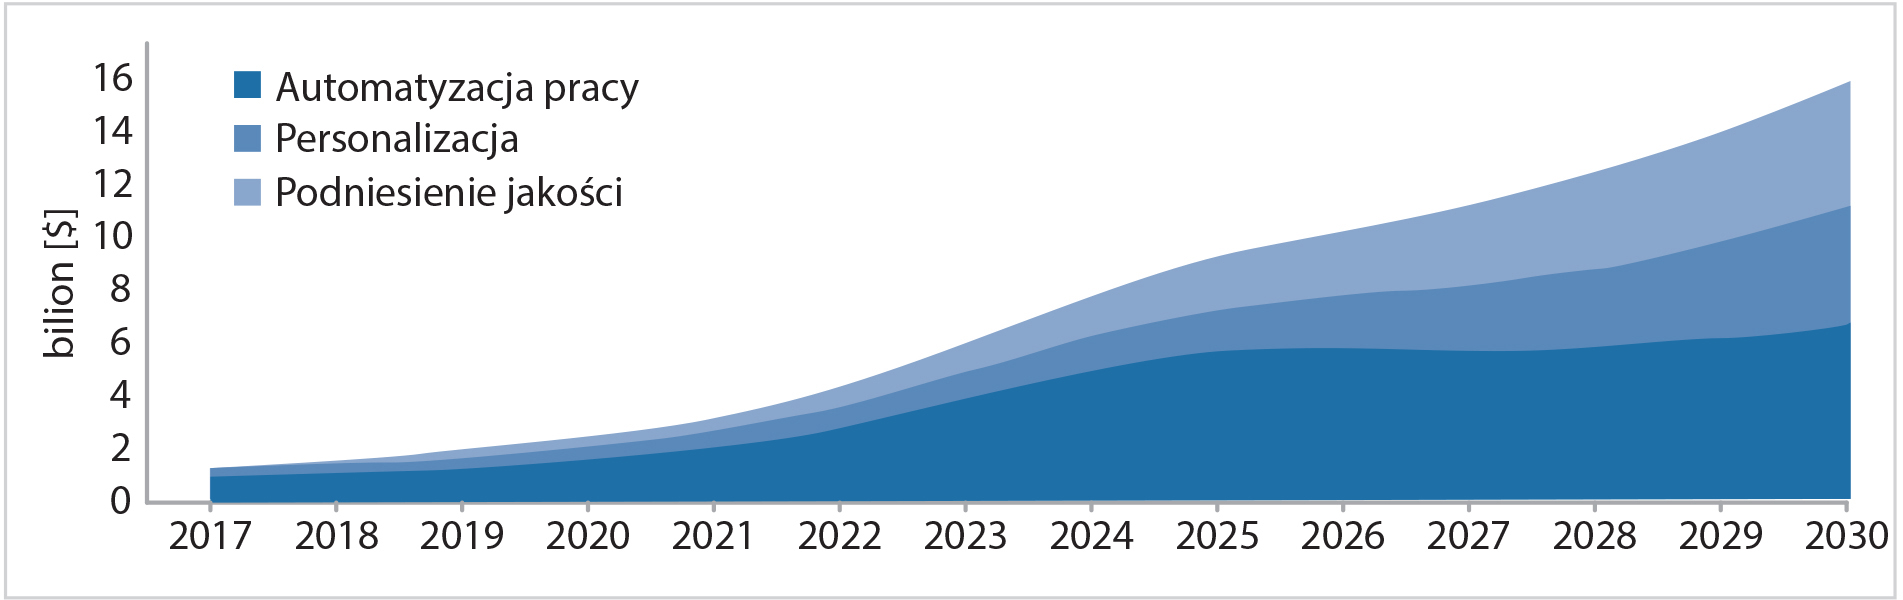
\includegraphics[width=1.0\textwidth]{figures/AI_w_radiologii.jpg}
	\caption{Kwota PKB wypracowana z udziałem rozwiązań opartych o SI aplikowanych na rynku Med-Tech (na podst. \cite{PWC}).}
	\label{MedTechGrowth}
\end{figure}

W pierwszej kolejności motorem zmian mają być aplikacje usprawniające generowanie raportów, następnie rozwiązania do personalizacji diagnostyki i narzędzia poprawiające jej jakość np. służące do uzyskania drugiej lub nawet pierwszej opinii. W rezultacie czas spędzony przez radiologa na pisanie raportu ma obniżyć się nawet o 90\%, przy niezmienionym lub nawet niższym współczynniku błędów diagnostycznych.

Metody, które według przewidywań mają najbardziej przyczynić się do rewolucji w radiologii, można podzielić na dwa rodzaje. Pierwszy to tzw. szeroka sztuczna inteligencja (ang. \textit{general Artificial Intelligence}), która docelowo ma odzwierciedlać złożony sposób zachowania się człowieka. Drugi rodzaj nazywany jest wąską Sztuczną Inteligencją (ang. \textit{narrow Artificial Intelligence}). Metody te mają zapewnić możliwie dobry efekt w wykonaniu konkretnego zadania np. klasyfikacji różnego rodzaju tkanek. 

W najbliższych latach przewidywane zmiany mają być efektem rozwoju metod wąskiej SI. Należy jednak podkreślić, że sam rozwój algorytmów ma już miejsce od ponad pół wieku. Krótki rys historyczny zawierający lata opracowania wybranych metod przedstawia się następująco: metoda regresji logistycznej -- rok 1958, ukryte modele Markova -- rok 1960, stochastyczny spadek wzdłuż gradientu -- rok 1960, Maszyna Wektorów Nośnych -- rok 1963, algorytm k-najbliższych sąsiadów -- rok 1967, wielowarstwowe sieci neuronowe -- lata 70-te ubiegłego wieku, algorytm EM (od ang. \textit{Expectation Maximization}) -- rok 1977, drzewa decyzyjne -- rok 1986, Q-learning -- rok 1989, lasy losowe -- rok 1995 oraz głębokie sieci neuronowych powstające \linebreak od lat 90-tych. 

W szczególności rozwój tych ostatnich został silnie przyspieszony z wykorzystaniem nowych architektur obliczeniowych takich jak akceleratory GPGPU (od ang. \textit{General-Purpose Computing on Graphics Processing Units}), czy TPU (od ang. \textit{Tensor Processing Unit}). Przede wszystkim uzyskano możliwość szybkiego testowania \linebreak i optymalizacji architektur zawierających miliony parametrów. W rezultacie dokładność realizacji przez współczesne metody bazujące na głębokich sieciach neuronowych, wybranych, praktycznych zadań, osiągnęła możliwości ludzkiej percepcji. 

\begin{figure}[h]
	\centering
	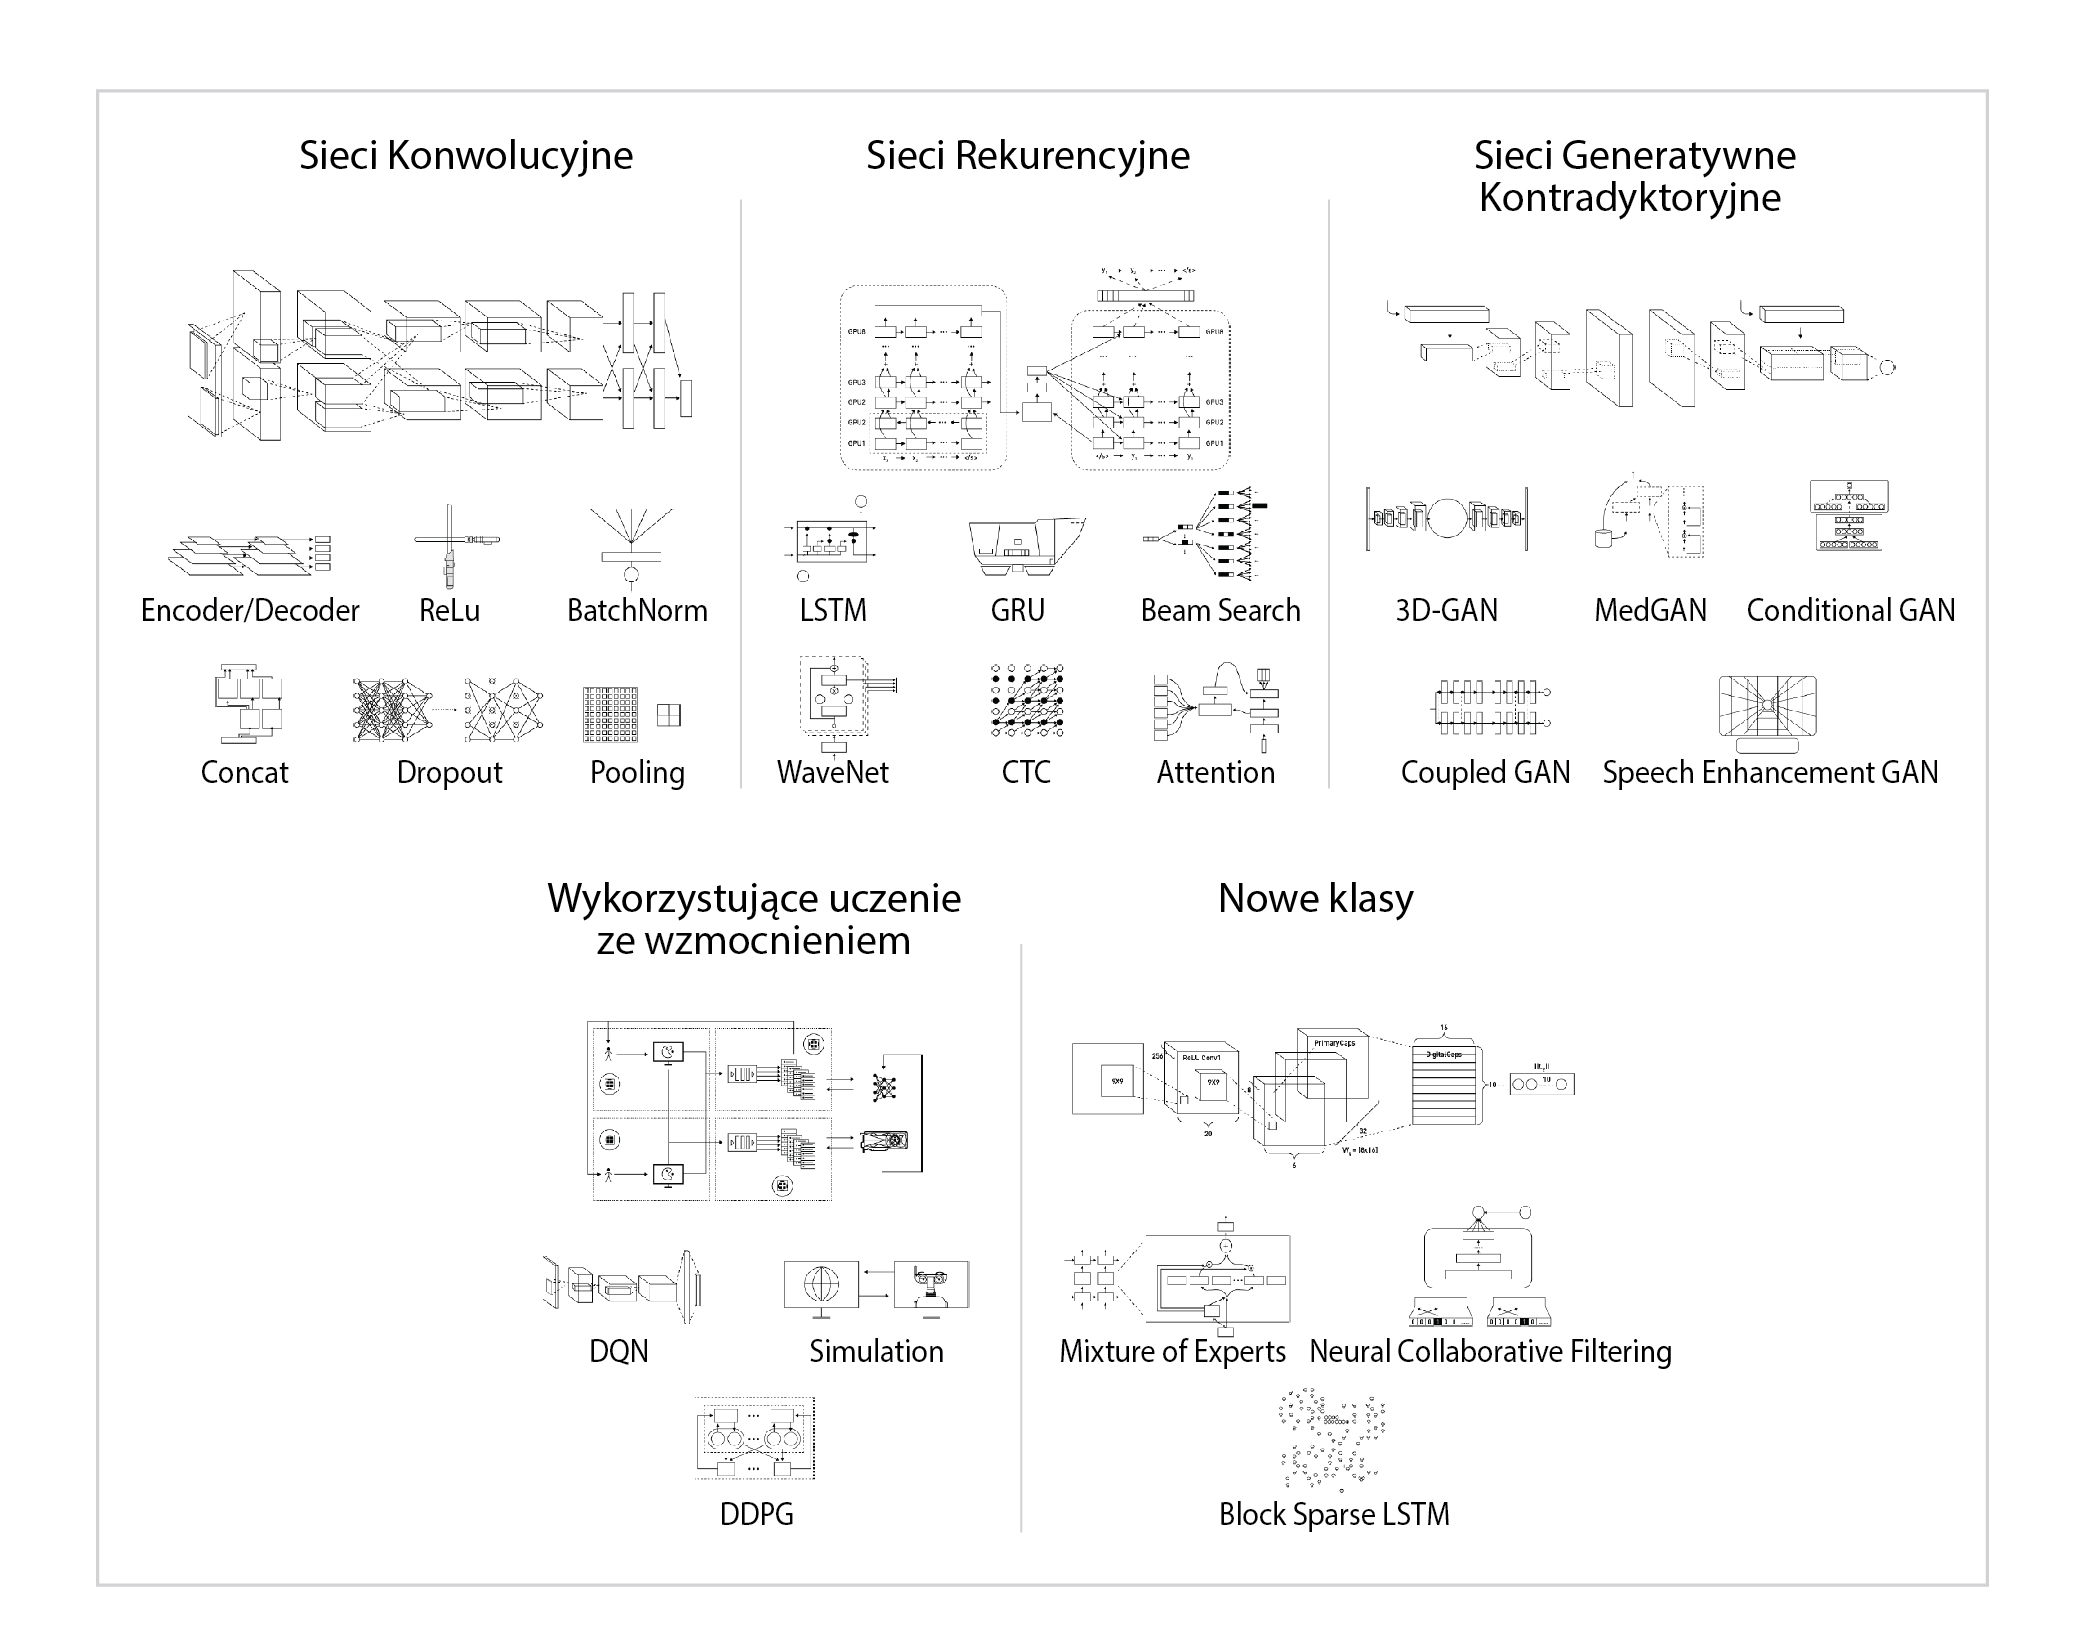
\includegraphics[width=1\textwidth]{figures/rodzajeSieciNeuronowych.png}
	\caption{Podział przedstawiający różne rodzaje współczesnych architektur głębokich sieci neuronowych.}
	\label{DLcambrianExplosion}
\end{figure}

Wśród głębokich sieci neuronowych wyróżnić można konwolucyjne sieci neuronowe stosowane najczęściej do przetwarzania obrazów, generatywne sieci kontradyktoryjne stosowane najczęściej do generowania danych, rekurencyjne sieci neuronowe stosowane najczęściej do rozpoznawania sekwencji, sieci wykorzystujące uczenie \linebreak ze wzmocnieniem do modelowania procesów decyzyjnych i szereg nowych klas jak sieci kapsułowe. Mnogość architektur (zob. Rys. \ref{DLcambrianExplosion}), powoduje, że na licznych konferencjach czy w publikacjach popularnonaukowych obecny stan rozwoju nazywany jest \textit{eksplozją kambryjską sieci neuronowych}. 


Z uwagi na fakt wykorzystania w radiologii w głównej mierze danych obrazowych, to właśnie konwolucyjne sieci neuronowe znajdują tu najczęstsze zastosowanie. Sieci te mają unikalną cechę umożliwiającą przekształcenia informacji obrazowej w numerycznie opisaną klasę przynależności. W szczególności, jak wskazują statystyki przedstawione na konferencji NVIDIA GTC w 2018 roku przez naukowców z niemieckiego centrum badań nad rakiem (DKFZ od niem. \textit{Deutsches Krebsforschungszentrum}), w około 71\% przypadków prace dotyczą automatycznego wydzielania struktur anatomicznych, w 12\% ich klasyfikacji, w 6\% samej detekcji (czy poszukiwane zjawisko znajduje się w danych) a w 3\% oceny postępu w leczeniu i monitoringu pacjentów. Pozostałe zadania jak np. lokalizowanie struktur, czy strukturyzacja danych przyjmują wartości poniżej 2\%.

W tej pracy, sieci konwolucyjne zostały wykorzystane do realizacji metody komputerowego wspomagania radiologa w zadaniu monitorowania pacjentów w trakcie rehabilitacji po przebytym urazie całkowitego zerwania ścięgna Achillesa. Zgodnie \linebreak z przedstawionymi powyżej statystykami, prace należą zatem do wąskiej grupy oceny leczenia i monitoringu. Ze względu na charakter obecnie realizowanych badań, stanowią nowatorskie podejście do przedmiotowego problemu i odpowiadają na istotne problemy w radiologii.


\chapter{Cel i struktura pracy}

Wyniki pracy zostały wykorzystane do realizacji projektu START: "Wykorzystanie autologicznych mezenchymalnych komórek macierzystych w procesie regeneracji rekonstruowanego ścięgna Achillesa", finansowanego przez Narodowe Centrum Badań i Rozwoju z krajowego programu STRATEGMED1. Celem całego projektu było "opracowanie nowych nieinwazyjnych technik obrazowania oraz metod monitorowania procesu regeneracji tkanek oraz ocena szybkości gojenia się ścięgna Achillesa". \linebreak W ramach tych prac powstała koncepcja automatyzacji procesu monitorowania gojenia się ścięgna przy pomocy metod przetwarzania obrazów i sztucznej inteligencji. Biorąc pod uwagę przedstawioną dalej budowę głębokich sieci neuronowych i ekstrahowane przez nie cechy, założono, że będą one skuteczne do oceny procesów patofizjologicznych widocznych w obrazowaniu medycznym takich jak gojenie tkanki miękkiej, co stanowi hipotezę tej pracy.

W ramach weryfikacji hipotezy, za cel główny autor tej pracy postanowił obrać opracowanie automatycznej metody oceny gojenia się ścięgna Achillesa, bazującej na fuzji danych z wykorzystaniem głębokich sieci neuronowych. Jako dane wejściowe postanowiono wykorzystać dane z Rezonansu Magnetycznego (RM), który jest rutynowo stosowany do obrazowania tkanek miękkich i z uwagi na podstawy fizyczne jest też dobrym wyborem do monitorowania gojenia tkanek, zwłaszcza z uwagi na zmiany w ich ukrwieniu podczas tego procesu. Wedle najlepszej wiedzy autora jest to pierwsza próba automatyzacji oceny gojenia się ścięgna Achillesa widocznego w obrazowaniu medycznym RM. Stąd konieczność zrealizowania celów pobocznych, które stanowią:
\begin{enumerate}[noitemsep,nolistsep]
	\item Wybór efektywnego kosztowo i czasowo protokołu badania bazującego na technikach obrazowania medycznego, a dokładniej Rezonansu Magnetycznego.
	\item Przetestowanie różnego rodzaju podejść związanych ze szkoleniem głębokich sieci neuronowych.
	\item Porównanie wyników oceny nowej metody z wynikami klasyfikacji bazującej na danych z ultrasonografii.
	\item Porównanie wyników oceny nowej metody z oceną funkcjonalną, rutynowo stosowaną do wspomagania rehabilitacji po urazie ścięgna.
\end{enumerate}

W celu uporządkowanego i zrozumiałego przedstawienia podłoża oraz wyników badań, w pracy wprowadzono podział na Rozdziały. Po wstępie i opisie celu pracy, w Rozdziale 3 zostały opisane współczesne metody monitorowania gojenia się ścięgna Achillesa. Rozdział ten rozpoczyna się od omówienia podstaw anatomicznych, biomechanicznych oraz dynamiki procesu gojenia się przedmiotowego ścięgna. Następnie przedstawiony jest szczegółowy opis badań obrazowych i biomechanicznych wykorzystywanych do oceny stanu rehabilitującego się pacjenta. W Rozdziale 4, omówione zostały szczegółowo konwolucyjne sieci neuronowe, które posłużyły jako rdzeń opracowanego rozwiązania. W szczególności, w opisie uwzględniono zarys historyczny pozwalający zrozumieć etapy rozwoju współczesnych sieci, problemy z budową efektywnych modeli na bazie sieci neuronowych oraz osiągnięcia w tym zakresie wraz z omówieniem sukcesów w zastosowaniach w medycynie. W Rozdziale 5 zaprezentowano nowatorską metodę automatycznej oceny procesu gojenia się ścięgna Achillesa. Co istotne, omówiono unikatowy zbiór danych oraz wzorzec odniesienia, dzięki którym możliwa była realizacja przewidzianych badań i walidacja metody. Przedstawiono również eksperymenty wykorzystane do doboru komponentów i parametrów ostatecznego modelu oraz finalny wynik funkcjonowania opracowanego algorytmu. W Rozdziale 6 opisano zestawienie wyników metody z wynikami oceny realizowanej przez inne podejścia. W szczególności porównano przedmiotową metodę z metodą uczącą się explicite modelować ocenę radiologa, opracowaną również pod kierownictwem autora tej pracy w ramach pobocznych działań. Następnie zaprezentowano zestawienie z wynikami metody działającej w oparciu o dane \linebreak z ultrasonografii, również opracowanej pod kierownictwem autora tej pracy. Finalnie, porównano wyniki z oceną biomechaniczną realizowaną standardowo przez fizjoterapeutów. Całość pracy zakończono podsumowaniem przedstawionym w Rozdziale~7.   



